\section{Overapproximation of Synchronous Traces} \label{sec:approach}
\alert{TODO: summary. main idea is to reduce bookkeeping as much as possible to improve scalability. note we use bool signals for convenience of demonstration, but the methods are general unless otherwise stated. finite signals obviously yield a finite alphabet. we use the values 0 and 1 for boolean signals. first describe a way of partitioning the temporal domain, then a way of encoding signals' behaviors as observed by the monitor and assigning them to these parts.}

STL$^+$ has the same syntax as STL and the below semantics.
$\tr^+(S,{\hb})$ is the overapproximation we compute.

\small
\begin{equation*}
	[(S,{\hb}) \models \varphi]_{\mathsf{STL}^+} = 
	\begin{cases}
		\top & \text{ if } \forall w \in \tr^+(S,{\hb}) : [w \models \varphi]_{\mathsf{STL}} \\
		\bot & \text{ if } \forall w \in \tr^+(S,{\hb}) : [w \models \lnot\varphi]_{\mathsf{STL}} \\
		\,? & \text{ otherwise}
	\end{cases}
\end{equation*}
\normalsize

\begin{theorem}
	For every STL formula $\varphi$ and every distributed signal $(S,{\hb})$, if $[(S,{\hb}) \models \varphi]_{\mathsf{STL}^+} = \top$ (resp. $\bot$) then $[(S,{\hb}) \models \varphi]_{\mathsf{STL}} = \top$ (resp. $\bot$).
\end{theorem}

\subsubsection{Canonical Segmentation}
Consider a boolean signal $x$ with a rising edge at time $t > \varepsilon$.
Due to clock skew, this edge occurs in the range $(t - \varepsilon, t + \varepsilon)$ from the monitor's point of view.
This range is called an \emph{uncertainty region} because in $(t - \varepsilon, t + \varepsilon)$ the monitor cannot tell the value of $x$ precisely, but only that it changes from 0 to 1.
Formally, given an edge $(t, x(t))$, we define $\theta_{\text{lo}}(x,t) = \max(0, t - \varepsilon)$ and $\theta_{\text{hi}}(x,t) = t + \varepsilon$ as the end points of the edge's uncertainty region.

Given a temporal domain $I = [0,d) \subset \R_{\geq 0}$, a \emph{segmentation} of $I$ is a partition of $I$ into finitely many intervals $I_1, \ldots, I_k$, called \emph{segments}, of the form $I_j = [t_j, t_{j+1})$ such that $t_j < t_{j+1}$ for all $1 \leq j \leq k$.
By extension, a segmentation of a collection of signals with the same temporal domain $I$ is a segmentation of $I$.

%Let $x : [0,d) \to \R$ be a signal and $(t, x(t))$ be an edge of $x$. %$E_x = \{(t_1, x(t_1)), \ldots, (t_m, x(t_m))\}$ be the set of edges of $x$, given in an increasing order of local clock values.
%We define $\theta_{\text{lo}}(x,t) = \max(0, t - \varepsilon)$ and $\theta_{\text{hi}}(x,t) = t + \varepsilon$.
%%\begin{align*}
%%	%	\theta_{\text{lo}}(x,t_i) &= \max\{0, \max_{j \in \{1, i\}} t_j - \varepsilon - (j-i)\delta\} \text{, and} \\
%%	\theta_{\text{lo}}(x,t_i) &= \max_{1 \leq j \leq i} t_j - \varepsilon + (i-j)\delta \text{, and} \\
%%	\theta_{\text{hi}}(x,t_i) &= \min_{i \leq j \leq m} t_j + \varepsilon - (j-i)\delta.
%%\end{align*}
%Intuitively, $\theta_{\text{lo}}$ and $\theta_{\text{hi}}$ give us the lower and upper bounds on the value of the monitor's clock for a given edge, i.e., the end points of the uncertainty region of the given edge.
%We use these to describe a canonical segmentation of a distributed signal.

Let $(S,{\hb})$ be a distributed signal of $n$ signals.
The \emph{canonical segmentation} $G_S$ of $(S,{\hb})$ is the segmentation of $S$ where the end points of the segments coincide with the end points of its edges' uncertainty regions.
Formally, we define $G_S$ as follows.
For each signal $x_i$, let $F_i$ be the set of end points of its uncertainty regions.
Let $d' = \max(d, \max (\bigcup_{i = 1}^{n} F_i))$, which corresponds to the duration of the distributed signal with respect to the monitor's clock.
%
Let $F = \{0, d'\} \cup \bigcup_{i = 1}^{n} F_i$ and let $(a_j)_{1 \leq j \leq |F|}$ be a nondecreasing sequence of clock values corresponding to the elements of $F$.
Then, the canonical segmentation of $(S,{\hb})$ is $G_S = \{I_1, \ldots, I_{|F| - 1}\}$ where $I_j = [a_j, a_{j+1})$ for all $1 \leq j < |F|$.

\begin{example} \label{ex:canonseg}
	\alert{TODO: canonical segmentation}
%	Let $(S, {\hb})$ be a distributed signal with $S = (x_1, x_2)$ over the temporal domain $[0,8)$ such that $\pi(x_1) \neq \pi(x_2)$.\borzoo{$\pi$ is unnecessary.}
%	Suppose $x_1(0) = 2$ and $x_2(0) = 3$, and let $\varepsilon = 2$ and $\delta = 3$.	
%	Consider the case where $x_1$ has a rising edge $(3,5)$ and a falling edge $(5,3)$ while $x_2$ has a rising edge $(2,7)$ and a falling edge $(5,2)$.
%	For $x_1$, taking into account only the clock skew would give us the uncertainty regions $(1,5)$ and $(3,7)$.\borzoo{We should this by a figure.}
%	However, the computation of uncertainty regions take into account also the bounded variability.
%	Intuitively, if the rising edge of $x_1$ occurs at global time 1, considering bounded variability, its falling edge occurs at the earliest at global time 4 instead of 3.
%	Conversely, if the falling edge occurs at global time 7 then its rising edge occurs at the latest at global time 4 instead of 5.
%	Then, we obtain $F_1 = \{1, 4, 7\}$.
%	For $x_2$, the uncertainty regions are $(0,4)$ and $(3,7)$, which gives us $F_2 = \{0, 3, 4, 7\}$; and therefore, $F_S = \{0, 1, 3, 4, 7, 8\}$.
%	This leads to the canonical segmentation $G_S = \{[0,1), [1,3) ,[3,4) ,[4,7) ,[7,8)\}$.		
\end{example}

\begin{figure} 
	\centering
	\caption{\alert{TODO}}
%	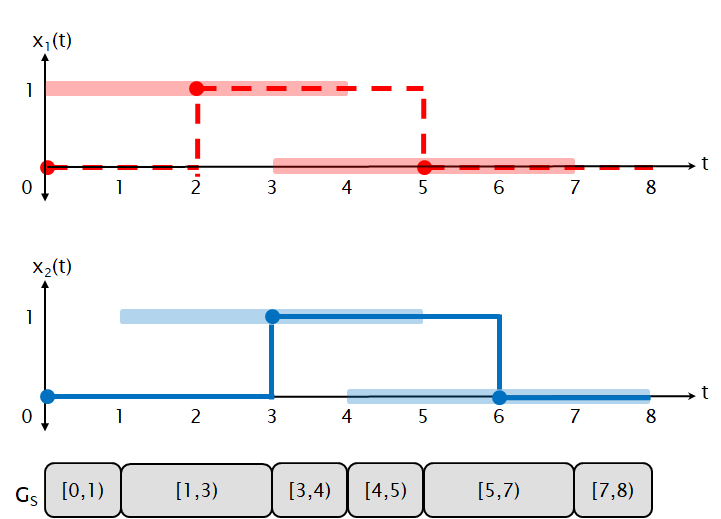
\includegraphics[scale=0.45]{canonseg.png}
%	\caption{The values of $x_1$ (solid) and $x_2$ (dashed) over time. The edges are marked with black balls and their uncertainty regions are given as light gray boxes around the edges. The resulting canonical segmentation $G_S$ is shown below the graphical representation of the signals.\label{fig:canonseg}}
	\label{fig:canonseg}
\end{figure}


\subsubsection{Value Expressions}
Consider a boolean signal $x$ with a rising edge with an uncertainty region of $(t_1, t_2)$.
As discussed above, the monitor only knows that the value of $x$ changes from 0 to 1 in this interval.
We represent this knowledge as a finite word $v = 0 \cdot 1$.
This representation is called a \emph{value expression} and it encodes the uncertain behavior of an observed signal relative to the monitor.
Formally, a value expression is an element of $\Sigma^*$ where $\Sigma$ is the finite alphabet of values the signal takes.
Given a signal $x$ and an edge $(t, x(t))$, the value expression corresponding to the uncertainty region $(\theta_{\text{lo}}(x,t), \theta_{\text{hi}}(x,t))$ is given by $v_{x,t} = v_- \cdot v_+$ where $v_- = \lim_{s \to t^-} x(s)$ and $v_+ = \lim_{s \to t^+} x(s)$.

Now, consider a distributed signal of two boolean signals $x_1$ and $x_2$ respectively with a rising edge in $(2,6)$ and a falling edge in $(4,8)$.
The corresponding value expressions are respectively $v_1 = 0 \cdot 1$ and $v_2 = 1 \cdot 0$.
Observe that, because the uncertainty regions intersect, the canonical segmentation of this distributed signal includes the segments $[2,4)$, $[4,6)$, and $[6,8)$.
The value expressions for these segments are obtained by prefixing and suffixing the original value expressions.
For example, since $[2,4)$ overlaps with $(2,6)$ from the left, the value expression for $[2,4)$ is given by $\pfx(v_1)$.


Formally, given a distributed signal $(S,{\hb})$, we define a function $\gamma : S \times G_S \to 2^{\Sigma^*}$ that maps each signal and segment of the canonical segmentation to a set of value expressions.
Let $x$ be a signal in $S$, and let $R_1, \ldots, R_m$ be its uncertainty regions where $R_i = (t_i, t_i')$ and the corresponding value expression is $v_i$ for all $1 \leq i \leq m$.
Now, let $I \in G_S$ be a segment with $I = [s, s')$ and for each $1 \leq i \leq m$ define the set $V_i$ of value expressions capturing how $I$ relates with $R_i$ as follows:

\small
\begin{equation*}
	V_i = 
	\begin{cases}
		\{v_i\} & \text{if } t_i = s \land s' = t_i' \\
		\pfx(v_i) & \text{if } t_i = s \land s' < t_i' \\
		\sfx(v_i) & \text{if } t_i > s \land s' = t_i' \\
		\infx(v_i) & \text{if } t_i > s \land s' < t_i' \\
		\{\epsilon\} & \text{otherwise}
	\end{cases}
\end{equation*}
\normalsize
Note that the last case happens only when $I \cap R_i$ is empty.
We finally define $\gamma(x,I) = \destutter(V_1 \cdot V_2 \cdot \ldots \cdot V_m) \setminus \{\epsilon\}$.
First, observe that $\gamma(x,I)$ contains all the potential behaviors of $x$ in segment $I$ by construction.
However, it is potentially overapproximate.
This is mainly because the sets $V_1, \ldots, V_m$ contain redundancy by definition and the concatenation may lead to taking some edges multiple times or never.
%We demonstrate an example in \cref{fig:valexpr}.

\begin{example} \label{ex:valexpr}
	\alert{TODO: value expressions and $\gamma$}
\end{example}

\begin{figure} 
	\centering
	\caption{\alert{TODO}}
	%	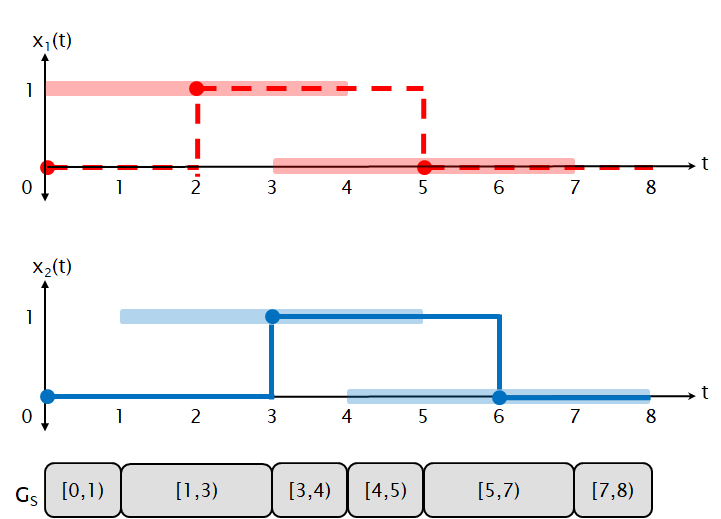
\includegraphics[scale=0.45]{canonseg.png}
	%	\caption{The values of $x_1$ (solid) and $x_2$ (dashed) over time. The edges are marked with black balls and their uncertainty regions are given as light gray boxes around the edges. The resulting canonical segmentation $G_S$ is shown below the graphical representation of the signals.\label{fig:canonseg}}
	\label{fig:valexpr}
\end{figure}



\subsubsection{Canonical Overapproximation of Traces}
Consider a distributed signal $(S,{\hb})$ of $n$ signals, and let $G_S$ be its canonical segmentation.
We describe how the function $\gamma$ defines a set $\tr^+(S,{\hb})$ of synchronous traces that overapproximates the set $\tr(S,{\hb})$.

Let $x \in S$ and $x'$ be two signals, and let $I = [s, s')$ be a segment in $G_S$.
Let $(t_1, x'(t_1)), \ldots, (t_\ell, x'(t_\ell))$ be the edges of $x'$ in segment $I$ such that $t_i < t_{i+1}$ for all $1 \leq i < \ell$.
The signals $x$ and $x'$ are \emph{consistent in $I$} iff $x(s) = x'(s)$ and the value expression $x'(t_1) \cdot \ldots \cdot x'(t_\ell)$ belongs to $\gamma(x,I)$.
Moreover, $x$ and $x'$ are \emph{consistent} iff they are consistent in $I$ for all $I \in G_S$.
Now, let $S = \{x_1, \ldots, x_n\}$ and define the \emph{canonical overapproximation} of $(S,{\hb})$ as follows:
$$ \tr^+(S,{\hb}) = \{ (x_1', \ldots, x_n') \st \text{$x_i$ and $x_i'$ are consistent for all $1 \leq i \leq n$}\} $$

\begin{lemma}
	For every distributed signal $(S,{\hb})$, we have $\tr(S,{\hb}) \subseteq \tr^+(S,{\hb})$.
\end{lemma}


\alert{
\begin{conjecture}
	Let $(S,{\hb})$ be a distributed signal with $|S| = 2$ and the maximum clock skew $\varepsilon$.
	Let ${\hb}'$ be happens-before relation obtained from ${\hb}$ by taking the maximum clock skew as $\varepsilon / 2$.
	Then, $\tr(S,{\hb}) \subseteq \tr^+(S,{\hb}')$.
\end{conjecture}
}